Son los dos tipos de señales sonoras (ejemplo en Fig. 4.2). Las señales mono se presentan en un solo canal, mientras que las estéreo presentan dos canales, izquierdo y derecho, por lo que crean una sensación espacial y de amplitud dinámica.

\begin{figure}[H]
    {\begin{center}
    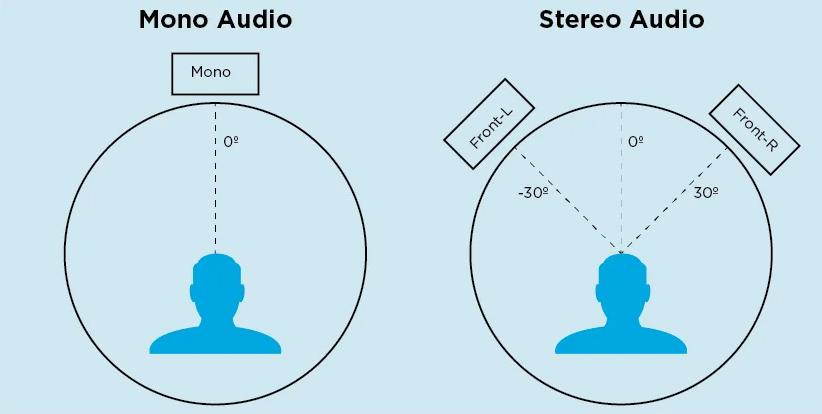
\includegraphics[width=0.7\textwidth]{commons/Fig2sound.jpg}
    \caption{Diferencia visual en una habitación entre un sonido mono y uno estéreo.}
    \label{fig:MonoEstereo}
    \end{center}}
\end{figure}
